\subsection{Bridge-Type Amplifier:}

In Figure 3.1.0 it's presented the differential instrumentation amplifier, after we assembled this circuit, we adjust the output voltage $V_{o}$ to zero volts with the preset help. As we can see we are using a {\itshape thermistor}, this device must be in ambient temperature, the measures consist in:

\begin{itemize}
\item Measure the output voltage with the {\itshape thermistor} in ambient temperature.
\item Measure the output voltage pressing with your fingers the {\itshape thermistor} to make it variate its temperature.
\item Measure the output voltage by putting very close to the {\itshape htermistor} lighter.
\end{itemize} \hfill

After measuring this output voltages, we capture our results in Table 1. \hfill \break

\begin{figure}[H]
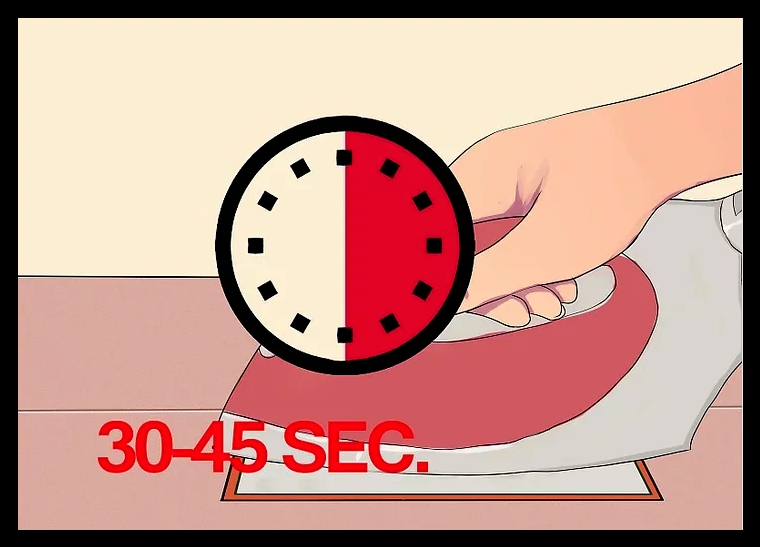
\includegraphics[width = 16.5cm, height = 8cm]{2.png}
\linebreak \linebreak \centering Figure 3.1.0: Instrumentation Amplifier.
\end{figure} \hfill \break

\begin{center}
\begin{tabular}{c c}
\toprule \toprule
\hspace{80px} Temperature \hspace{80px} & \hspace{80px} Output Voltage \hspace{80px} \\
\midrule \midrule
Ambient & 0.40 mV \\
\cmidrule{1-2}
Pressing with fingers & 0.96 V \\
\cmidrule{1-2}
Putting a lighter close & 2.21 V \\
\bottomrule
\end{tabular}
\linebreak \linebreak Table 1: Figure 3.1.0 measured values.
\end{center}

\pagebreak